%%%%%%%%%%%%%%%%%%%%%%%%%%%%%%%%%%%%%%%%%

%----------------------------------------------------------------------------------------
%	TITLE SLIDE
%----------------------------------------------------------------------------------------
\documentclass{beamer}
\definecolor{myGold}{RGB}{255,255,255}
\definecolor{cadmiumgreen}{rgb}{0.0, 0.42, 0.24}
\setbeamercolor{structure}{fg=cadmiumgreen}
\setbeamercolor{normal text}{fg=myGold}
\usetheme{Warsaw}
\usepackage{multicol}
\usepackage{textpos}
\usepackage{epigraph}
\usepackage{dirtytalk}
\usepackage{textcomp}
\addtobeamertemplate{frametitle}{}{%
\begin{textblock*}{200mm}(.98\textwidth,-1cm)

\includegraphics[height=1cm,width=1cm]{cdac1.png}
\end{textblock*}}
\begin{document}
\setbeamertemplate{background canvas}{
\includegraphics[width=\paperwidth,height=\paperheight]{2.png}}

\title[Django]{Django}  
%\subtitle{Classification\\\includegraphics[height=1cm,width=2cm]{ml2.png}}
%\author{\includegraphics[height=.2cm,width=1cm]{cdaclogo.png}
%\includegraphics[height=.2cm,width=1cm]{cdaclogoe.png}
\author[STDC]{STDC}
\date{\today} 
\maketitle
\frame{\frametitle{Table of contents} 
    \begin{multicols*}{2}
    \small{\tableofcontents}
    \end{multicols*}
    }


%----------------------------------------------------------------------------------------
%	PRESENTATION BODY SLIDES
%----------------------------------------------------------------------------------------

%\section{Python} % Sections are added in order to organize your presentation into discrete blocks, all sections and subsections are automatically output to the table of contents as an overview of the talk but NOT output in the presentation as separate slides

%------------------------------------------------
\section{Django Web Framework (Python)}
\subsection{Server-side website programming}
\begin{frame}
	\frametitle{Server-side website programming}
 \begin{itemize}
    \item Django is an extremely popular and fully featured server-side web framework, written in Python. 
    \item Web browsers communicate with web servers using the HyperText Transfer Protocol (HTTP). 
    \item When click a link on a web page, submit a form, or run a search, an HTTP request is sent from your browser to the target server.
\end{itemize} 	
\end{frame}
%------------------------------------------------
\begin{frame}
	\frametitle{Server-side website programming}
 \begin{itemize}
    \item The request includes a URL identifying the affected resource, a method that defines the required action (for example to get, delete, or post the resource), and may include additional information encoded in URL parameters (the field-value pairs sent via a query string), as POST data (data sent by the HTTP POST method), or in associated cookies.
\end{itemize} 	
\end{frame}
%------------------------------------------------
%\subsection{Classification}
\begin{frame}
\frametitle{Static sites}
\begin{itemize}
    \item When a user wants to navigate to a page, the browser sends an HTTP "GET" request specifying its URL.
\item The server retrieves the requested document from its file system and returns an HTTP response containing the document and a success status (usually 200 OK). 
\item If the file cannot be retrieved for some reason, an error status is returned.
\end{itemize}
\end{frame}
%------------------------------------------------
\begin{frame}
\frametitle{Static sites}
\begin{figure}
	    \centering
	    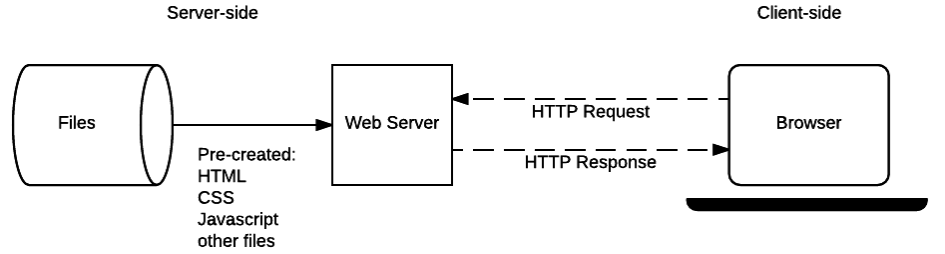
\includegraphics[height=5cm,width=11cm]{l1.png}
	    %\caption{Caption}
	   %\label{fig:my_label}
	\end{figure}
\end{frame}
%------------------------------------------------
\begin{frame}
\frametitle{Dynamic sites}
\begin{itemize}
    \item A dynamic website is one where some of the response content is generated dynamically, only when needed. 
    \item On a dynamic website, HTML pages are normally created by inserting data from a database into placeholders in HTML templates.
\item A dynamic site can return different data for a URL based on information provided by the user or stored preferences and can perform other operations as part of returning a response.
\item Most of the code to support a dynamic website must run on the server. Creating this code is known as "server-side programming".
\end{itemize}
\end{frame}
%------------------------------------------------
\begin{frame}
\frametitle{Dynamic sites}
\begin{figure}
	    \centering
	    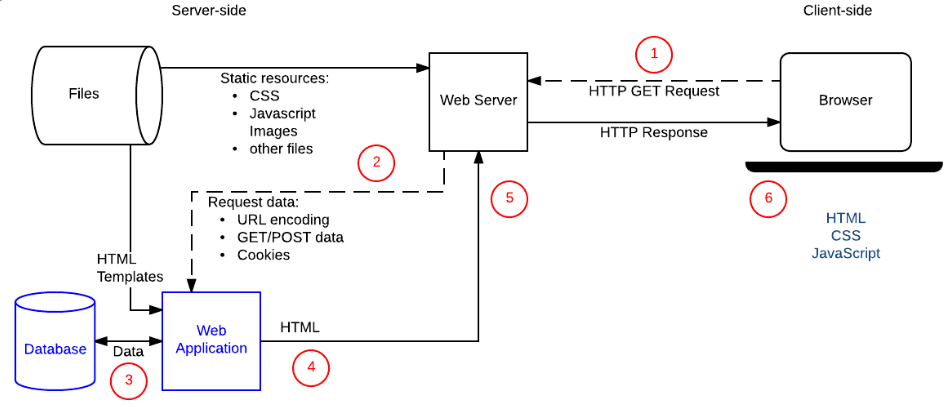
\includegraphics[height=5cm,width=11cm]{l2.png}
	    %\caption{Caption}
	   %\label{fig:my_label}
	\end{figure}
\end{frame}
%------------------------------------------------
\begin{frame}
\frametitle{Dynamic sites}
\begin{itemize}
    \item Server-side programming allows sites to restrict access to authorized users and serve only the information that a user is permitted to see.
    \item Server-side programming allows developers to make use of sessions — a mechanism that allows a server to store information associated with the current user of a site and send different responses based on that information.
\end{itemize}
\end{frame}
%------------------------------------------------
\subsection{Web servers and HTTP }
\begin{frame}
\frametitle{Web servers and HTTP }
\begin{itemize}
    \item Web browsers communicate with web servers using the HyperText Transfer Protocol (HTTP). 
    \item When you click a link on a web page, submit a form, or run a search, the browser sends an HTTP Request to the server.
  \end{itemize}
\end{frame}
%------------------------------------------------
\begin{frame}
\frametitle{Web servers and HTTP }
\begin{itemize}
    \item The request includes:
    \begin{itemize}
    \item When you click a link on a web page, submit a form, or run a search, the browser sends an HTTP Request to the server.
    \item A method that defines the required action (for example, to get a file or to save or update some data). 
  \end{itemize}
  \end{itemize}
\end{frame}
%------------------------------------------------
\begin{frame}
\frametitle{Web servers and HTTP }
\begin{itemize}
 \item GET: Get a specific resource.
\item POST: Create a new resource.
\item HEAD: Get the metadata information about a specific resource without getting the body like GET would. 
\item PUT: Update an existing resource.
\item DELETE: Delete the specified resource.
   \end{itemize}
\end{frame}
%------------------------------------------------

\begin{frame}
\frametitle{Web servers and HTTP }
\begin{itemize}
 \item The web browser creates an HTTP GET request to the server using the base URL for the resource and encoding the team and player number either as URL parameters or as part of the URL pattern. 
 \item A GET request is used because the request is only fetching data (not modifying data).
   \end{itemize}
\end{frame}
%------------------------------------------------
\begin{frame}
\frametitle{Web servers and HTTP }
\begin{itemize}
 \item The Web Application identifies that the intention of the request is to get the "best team list" based on the URL (/best/) and finds out the required team name and number of players from the URL. 
 \item The Web Application then gets the required information from the database.
   \end{itemize}
\end{frame}
%------------------------------------------------
\subsection{Django Framework}
\begin{frame}
\frametitle{A web framework - Django }
\begin{itemize}
 \item Web frameworks provide tools and libraries to simplify common web development operations.
 \item Django is a high-level Python Web framework that encourages rapid development and clean, pragmatic design. 
 \item Popular sites using Django (from Django home page) include: Disqus, Instagram, Knight Foundation, MacArthur Foundation, Mozilla, National Geographic, Open Knowledge Foundation, Pinterest, Open Stack.
   \end{itemize}
\end{frame}
%------------------------------------------------
\begin{frame}
\frametitle{A web framework - Django }
\begin{figure}
	    \centering
	    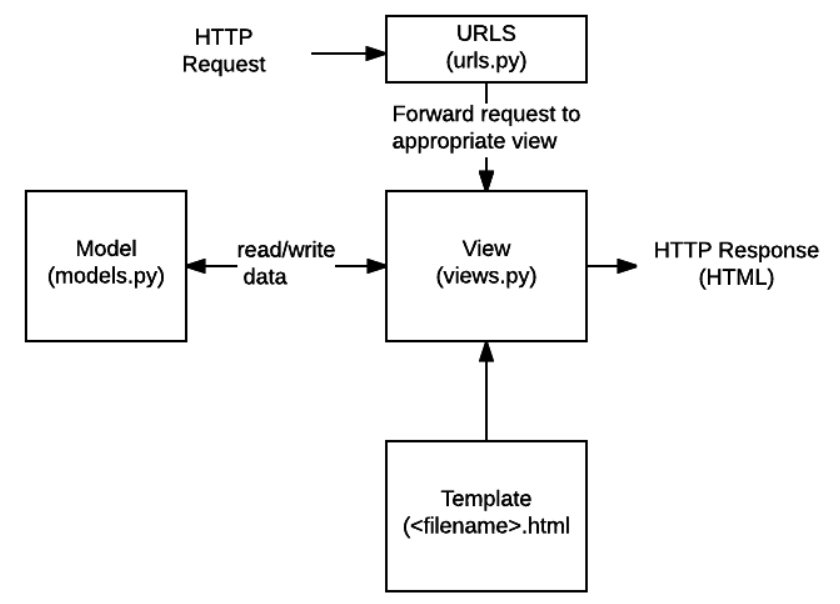
\includegraphics[height=6cm,width=11cm]{l3.png}
	    %\caption{Caption}
	   %\label{fig:my_label}
	\end{figure}
\end{frame}
%------------------------------------------------
\begin{frame}
\frametitle{Django-URLs }
\begin{itemize}
 \item While it is possible to process requests from every single URL via a single function, it is much more maintainable to write a separate view function to handle each resource. 
 \item A URL mapper is used to redirect HTTP requests to the appropriate view based on the request URL. 
 \item The URL mapper can also match particular patterns of strings or digits that appear in a URL and pass these to a view function as data.
   \end{itemize}
\end{frame}
%------------------------------------------------
\begin{frame}
\frametitle{Django-View}
\begin{itemize}
 \item A view is a request handler function, which receives HTTP requests and returns HTTP responses. 
 \item Views access the data needed to satisfy requests via models, and delegate the formatting of the response to templates.
   \end{itemize}
\end{frame}
%------------------------------------------------
\begin{frame}
\frametitle{Django-Models}
\begin{itemize}
 \item Models are Python objects that define the structure of an application's data, and provide mechanisms to manage (add, modify, delete) and query records in the database.
   \end{itemize}
\end{frame}
%------------------------------------------------
\begin{frame}
\frametitle{Django-Templates}
\begin{itemize}
 \item A template is a text file defining the structure or layout of a file (such as an HTML page), with placeholders used to represent actual content. 
 \item A view can dynamically create an HTML page using an HTML template, populating it with data from a model. 
 \item A template can be used to define the structure of any type of file; it doesn't have to be HTML!
   \end{itemize}
\end{frame}
%------------------------------------------------
\subsection{HTML}
\begin{frame}
\frametitle{HTML}
\begin{itemize}
 \item HTML is the standard markup language for creating Web pages.
 \item HTML stands for Hyper Text Markup Language
\item HTML describes the structure of a Web page
\item HTML consists of a series of elements
\item HTML elements tell the browser how to display the content
\item HTML elements label pieces of content such as "this is a heading", "this is a paragraph", "this is a link", etc.
\end{itemize}
\end{frame}
%------------------------------------------------
\begin{frame}
\frametitle{HTML}
\begin{itemize}
 \item The $<$ !DOCTYPE html$>$ declaration defines that this document is an HTML5 document
\item The $<$html$>$ element is the root element of an HTML page
\item The $<$head$>$ element contains meta information about the HTML page
\item The $<$title$>$ element specifies a title for the HTML page (which is shown in the browser's title bar or in the page's tab)
\item The $<$body$>$ element defines the document's body, and is a container for all the visible contents, such as headings, paragraphs, images, hyperlinks, tables, lists, etc.
\item The $<$h1$>$ element defines a large heading
\item The $<$p$>$ element defines a paragraph

\end{itemize}
\end{frame}
%------------------------------------------------
\begin{frame}
\frametitle{Formatting}
\begin{itemize}
 \item   $<$p$>$ $<$/p$>$:  Creates a new paragraph
 \item   $<$br$>$:  AInserts a line break (carriage return)
  \item  $<$blockquote$>$ $<$/blockquote$>$:  Puts content in a quote - indents text from both sides
  \item  $<$div$>$ $<$/div$>$: Used to format block content with CSS
  \item  $<$span$>$ $<$/span$>$: Used to format inline content with CSS
\end{itemize}
\end{frame}
%------------------------------------------------
\begin{frame}
\frametitle{Body attributes}
\begin{itemize}
 \item  $<$body bgcolor=?$>$: Sets background color, using name or hex value
\item  $<$body text=?$>$:  Sets text color, using name or hex value
\item  $<$body link=?$>$:  Sets color of links, using name or hex value
\item  $<$body vlink=?$>$:  Sets color of visited links, using name or hex value
\item  $<$body alink=?$>$: Sets color of active links (while mouse-clicking)
\end{itemize}
\end{frame}
%------------------------------------------------
\begin{frame}
\frametitle{ Text Tags}
\begin{itemize}
 \item  $<$pre$>$ $<$/pre$>$
 Creates preformatted text
 \item  $<$h1$>$ $<$/h1$>$ --$>$ $<$h6$>$ $<$/h6$>$
 Creates headlines -- H1=largest, H6=smallest
 \item  $<$b$>$ $<$/b$>$
 Creates bold text (should use $<$strong$>$ instead)
 \item  $<$i$>$ $<$/i$>$
 Creates italicized text (should use $<$em$>$ instead)
 \item  $<$tt$>$ $<$/tt$>$
 Creates typewriter-style text
\item   $<$code$>$ $<$/code$>$
 Used to define source code, usually monospace
 \item  $<$cite$>$ $<$/cite$>$
 Creates a citation, usually processed in italics
 \item  $<$address$>$ $<$/address$>$
 Creates address section, usually processed in italics
 \end{itemize}
\end{frame}
%------------------------------------------------
\begin{frame}
\frametitle{ Text Tags}
\begin{itemize}
  \item  $<$em$>$ $<$/em$>$
 Emphasizes a word (usually processed in italics)
 \item  $<$strong$>$ $<$/strong$>$
 Emphasizes a word (usually processed in bold)
 \item  $<$font size=?$>$ $<$/font$>$    
Sets size of font - 1 to 7 (should use CSS instead)
 \item  $<$font color=?$>$ $<$/font$>$
 Sets font color (should use CSS instead)
 \item  $<$font face=?$>$ $<$/font$>$
 Defines the font used (should use CSS instead)
\end{itemize}
\end{frame}
%------------------------------------------------
\begin{frame}
\frametitle{ Lists}
\begin{itemize}
  \item   $<$ul$>$ $<$/ul$>$:  Creates an unordered list
\item $<$ol start=?$>$ $<$/ol$>$:  Creates an ordered list (start=xx,
 where xx is a counting number)
 \item $<$li$>$ $<$/li$>$:  Encompasses each list item
 \item $<$dl$>$ $<$/dl$>$:  Creates a definition list
 \item $<$dt$>$:      Precedes each defintion term
 \item $<$dd$>$:     Precedes each definition
\end{itemize}
\end{frame}
%------------------------------------------------
\begin{frame}
\frametitle{ Links}
\begin{itemize}
  \item    $<$a href="URL"$>$clickable text$<$/a$>$: Creates a hyperlink to a Uniform Resource Locator
 \item $<$a href="mailto:EMAIL\_ADDRESS"$>$clickable text$<$/a$>$:
 Creates a hyperlink to an email address
 \item $<$a name="NAME"$>$:  Creates a target location within a document
 \item $<$a href="\#NAME"$>$clickable text$<$/a$>$:  Creates a link to that target location
\end{itemize}
\end{frame}
%------------------------------------------------
\begin{frame}
\frametitle{Graphical elements}
\begin{itemize}
  \item   $<$hr$>$:  Inserts a horizontal rule
 \item $<$hr size=?$>$:  Sets size (height) of horizontal rule
 \item $<$hr width=?$>$:  Sets width of rule (as a \% or absolute pixel length)
 \item $<$hr noshade$>$:  Creates a horizontal rule without a shadow
 \item $<$img src="URL" /$>$:  Adds image; it is a separate file located at the URL
 \item $<$img src="URL" align=?$>$:  Aligns image left/right/center/bottom/top/middle (use CSS)
 \end{itemize}
\end{frame}
%------------------------------------------------
\begin{frame}
\frametitle{Graphical elements}
\begin{itemize}
  \item  $<$img src="URL" border=?$>$:  Sets size of border surrounding image (use CSS)
  \item  $<$img src="URL" height=?$>$:  Sets height of image, in pixels
 \item   $<$img src="URL" width=?$>$:  Sets width of image, in pixels
  \item  $<$img src="URL" alt=?$>$:  Sets the alternate text for browsers that can't
 process images 
\end{itemize}
\end{frame}
%------------------------------------------------
\begin{frame}
\frametitle{Forms}
\begin{itemize}
  \item   $<$form$>$ $<$/form$>$:  Defines a form
 \item   $<$select multiple name=? size=?$>$ $<$/select$>$:  Creates a scrolling menu. Size sets the number of
 menu items visible before user needs to scroll.
 \item   $<$select name=?$>$ $<$/select$>$:  Creates a pulldown menu
 \item   $<$option$>$:  Sets off each menu item
 \item   $<$textarea name=? cols="x" rows="y"$>$$<$/textarea$>$:  Creates a text box area. Columns set the width;
 rows set the height.
\end{itemize}
\end{frame}
%------------------------------------------------
\begin{frame}
\frametitle{Forms}
\begin{itemize}
  \item   $<$input type="checkbox" name=? value=?$>$:  Creates a checkbox.
 \item   $<$input type="checkbox" name=? value=? checked$>$:  Creates a checkbox which is pre-checked.
 \item   $<$input type="radio" name=? value=?$>$:  Creates a radio button.
\item    $<$input type="radio" name=? value=? checked$>$:  Creates a radio button which is pre-checked.
 \item   $<$input type="text" name=? size=?$>$:  Creates a one-line text area.  Size sets length, in characters.
\end{itemize}
\end{frame}
%------------------------------------------------
\begin{frame}
\frametitle{Forms}
\begin{itemize}
  \item   $<$input type="submit" value=?$>$:  Creates a submit button.  Value sets the text in the  submit button.
  \item   $<$input type="image" name=? src=? border=? alt=?$>$:  Creates a submit button using an image. 
 \item   $<$input type="reset"$>$:  Creates a reset button
\end{itemize}
\end{frame}
%------------------------------------------------
\begin{frame}
\frametitle{Tables}
\begin{itemize}
  \item   $<$table$>$ $<$/table$>$:  Creates a table
   \item   $<$tr$>$ $<$/tr$>$:  Sets off each row in a table
  \item    $<$td$>$ $<$/td$>$:  Sets off each cell in a row
   \item   $<$th$>$ $<$/th$>$:  Sets off the table header (a normal cell with bold,
 centered text)
\end{itemize}
\end{frame}
%------------------------------------------------
\begin{frame}
\frametitle{Table attributes }
\begin{itemize}
  \item    $<$table border=?$>$:  Sets the width of the border around table cells
  \item   $<$table cellspacing=?$>$:  Sets amount of space between table cells
  \item   $<$table cellpadding=?$>$:  Sets amount of space between a cell's border and  its contents
  \item   $<$table width=?$>$:  Sets width of the table in pixels or as a percentage
\end{itemize}
\end{frame}
%------------------------------------------------
\begin{frame}
\frametitle{Table attributes }
\begin{itemize}
  \item    $<$tr align=?$>$:  Sets alignment for cells within the row
 (left/center/right)
 \item     $<$td align=?$>$:  Sets alignment for cells (left/center/right)
 \item     $<$tr valign=?$>$:  Sets vertical alignment for cells within the row
 (top/middle/bottom)
 \item     $<$td valign=?$>$:  Sets vertical alignment for cell (top/middle/bottom)
  \item    $<$td rowspan=?$>$:  Sets number of rows a cell should span (default=1)
  \item    $<$td colspan=?$>$:  Sets number of columns a cell should span
  \item    $<$td nowrap$>$:  Prevents lines within a cell from being broken to fit
\end{itemize}
\end{frame}
%------------------------------------------------
\begin{frame}
\frametitle{HTML5 input tag attributes  }
\begin{itemize}
  \item   $<$input type="email" name=?$>$ :                Sets a single-line textbox for email addresses 
 \item  $<$input type="url" name=?$>$ :     Sets a single-line textbox for URLs 
 \item  $<$input type="number" name=?$>$:      Sets a single-line textbox for a number 
 \item  $<$input type="range" name=?$>$ :    Sets a single-line text box for a range of numbers 
 \item  $<$input type="date/month/week/time" name=?$>$:      Sets a single-line text box with a calendar  
     showing the date/month/week/time 
 \item  $<$input type="search" name=?$>$ :      Sets a single-line text box for searching 
 \item  $<$input type="color" name=?$>$ :      Sets a single-line text box for picking a color
\end{itemize}
\end{frame}
%------------------------------------------------
\end{document}
%------------------------------------------------